\section{Results} \label{sec:simulation}

Here we present a simulation-based evaluation of the \textsc{stam} and \textsc{stfu} schedulers. 
% by classic compafrom non-smoothed task lists.  Our simulation includes a stochastic energy harvesting process, a random task list and \textsc{stam}/\textsc{stfu} task list generator, the scheduling processes, and an execution process.  We execute $n$ simulations on one task list per run, and generate task lists for $r$ runs.  Each task list consists of $k$ tasks.

\subsection{Simulator Details }

\begin{figure}[htb]
\begin{center}
\caption{Markov Chain Weather Model.\label{fig:markov}}
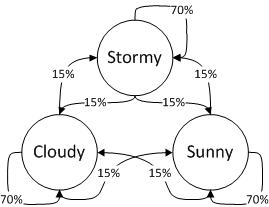
\includegraphics[scale=0.8]{markov.png}
\end{center}
\end{figure}
\begin{table}[h]
\begin{center}

\begin{tabular}{| l | l || l | l |}
\hline
\textbf{$G$ ($\frac{W}{m^2}$)} & \textbf{$I_c$ ($A$)} & \textbf{$G$ ($\frac{W}{m^2}$)} & \textbf{$I_c$ ($A$)} \\
\hline
\textbf{50} & \textbf{0.190} & 175 & 0.665 \\
75 & 0.285 & \textbf{200} & \textbf{0.760} \\
\textbf{100} & \textbf{0.380} & 225 & 0.855 \\
125 & 0.475 & 250 & 0.950 \\
150 & 0.570 & 275 & 1.045 \\
\hline
\end{tabular}
\end{center}
\caption{Solar panel energy output (bold values are used in our weather model)\label{tab:radiance}}
\end{table}

Our simulation framework includes a stochastic energy harvesting process, a task list generator, the scheduling processes, and an execution process.  
We execute $n$ simulations on one task list per run, and generate task lists for $r$ runs.  Each task list consists of $k$ tasks.

%We execute $n$ simulations on one task list per run, and generate task lists for $r$ runs.  Each task list consists of $k$ tasks.
%We have developed a simulation framework for comparing schedules generated from \textsc{stam} and \textsc{stfu} task lists to schedules generated from non-smoothed task lists.  Our simulation includes a stochastic energy harvesting process, a random task list and \textsc{stam}/\textsc{stfu} task list generator, the scheduling processes, and an execution process.  We execute $n$ simulations on one task list per run, and generate task lists for $r$ runs.  Each task list consists of $k$ tasks.

%\subsection{Task Generation}
The tasks are generated with random periods, durations, and energy requirements.  The periods and durations are distributed uniformly in discrete time steps, 
ranging respectively from 10 to 40 and from 1 to 4.  
The energy is half-normally distributed, and proportional to the task's period (\emph{i.e.} a task requiring high energy is expected to run at a low frequency).

We consider only task lists that are \emph{temporally schedulable} which we define as having a 
CPU utilization $U$ less than 100\% (see Equation \ref{eqn:utilization}). 
For each task list we also generate a corresponding virtual task list using \textsc{stam} and \textsc{stfu}. 

%\subsection{Energy Harvesting Model}

We use the model of a photovoltaic energy harvester, which converts solar irradiance $G$ into a current $I_c$, as a stochastic energy source for our simulation.  The energy drawn from the environment is modeled as a 3-state Markov chain (\cite{poggi2000stochastic,moser2007real}) representing three weather conditions (Figure~\ref{fig:markov}).  At each discrete time step during the simulation the Markov chain is updated, and the energy generated added to an energy pool (\emph{i.e.} a battery).

We generated a table of energy inputs to the system using the solar cell model provided by 
Simulink's SimElectronics toolkit, configured with values from \cite{gonzalez2006model}.  
The solar cell's current output with a battery load is related to its radiation input as 
determined by the linear function $I_c = 0.0038G$.  
We use the values of $G = 50, 100, 200 \frac{W}{m^2}$ to represent stormy, cloudy, and sunny weather conditions 
in our weather model.

The output current of the photovoltaic cell, $I_c$, is governed by a two-diode formula given in \cite{marwali1997probabilistic} and modeled by the Simulink model.  
The current flows into a battery, which we simulate using a linear model without relaxation effect.  
The battery capacity at time $t$, $B_t$ is calculated using equation~\ref{eqn:batterycharge} per \cite{niyato2007sleep}.
\begin{equation}
 B_t = B_{t-1} + I_c \Delta t - I_d \Delta t
\label{eqn:batterycharge}
\end{equation}
where 
\begin{description}
\item[$B_{t-1}$] is the previous battery capacity
\item[$I_c$] is the charge current due to solar harvesting during $\Delta t$
\item[$I_d$] is the discharge current due to task execution during $\Delta t$
\end{description}
We represent $I_c$ and $I_d$  as constant averages during the interval $\Delta t$. Furthermore, the battery is
limited in capacity, such that if $B_t = B_{max}$ then any excess energy that is harvested is lost.

\subsection{Simulation Results}

\begin{figure}[tb]
\begin{center}
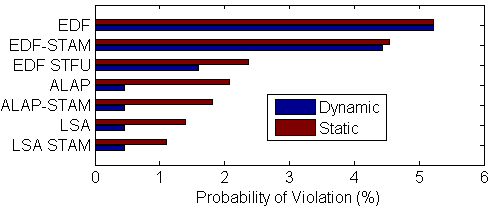
\includegraphics[scale=0.65]{bar.png}
\end{center}
\caption{Violations rate with and without dynamic task rescheduling; 
results averaged from 1000 task lists of less than 50\% utilization.  \label{fig:simresults}}
\end{figure}

\begin{figure}[tb]
\begin{center}
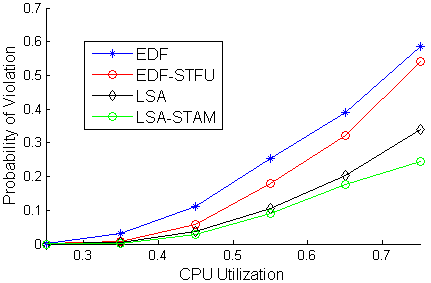
\includegraphics[scale=0.57]{violations_vs_cpuutil.png}
\caption{
Violation probability computed over 100 simulations, as a function of physical task utilization for static schedulers.\label{fig:violations_vs_cpuutil}
}
\end{center}
\end{figure}

%\subsubsection{Static Scheduling}

For performance evaluation we 
used earliest-deadline-first (\textsc{edf}) and as-late-as-possible (\textsc{alap}) scheduling to schedule real tasks, \textsc{stam} virtual tasks, and \textsc{stfu} virtual tasks. 
In \textsc{edf}, each task is scheduled as early as possible, in order of increasing deadline.  
In \textsc{alap}, tasks are scheduled at the latest time possible such that no task misses its deadline.  

For comparison purposes, we implemented \emph{dynamic} Lazy Scheduling Algorithm (\textsc{lsa}) 
as described by Moser \emph{et al.} \cite{moser2007real}.  
\footnote{We implement \textsc{lsa-i} as described in that paper} 
Additionally, we implemented a \emph{static} Lazy Scheduling Algorithm (\textsc{lsa}) that incorporates 
an off-line prediction of when the battery is at capacity. 
To create a static \textsc{lsa} schedule we pre-process an \textsc{alap} schedule using our dynamic simulation routine, with a constant minimal energy input in place of the stochastic input.  This constant input is the prediction we give to \textsc{lsa}.  As a result, in \textsc{lsa} tasks will be statically rescheduled when the model can guarantee that the battery is at maximum capacity, \emph{e.g.} at the start of the simulation before any tasks have run.  Energy may still be wasted in the static-schedule, stochastic simulation model when the battery reaches its maximum capacity unexpectedly.  
%The only way to avoid that would be to predict the energy input while generating the static schedule.

Although our focus is on static scheduling, we also implemented \emph{dynamic} versions of each of the schedulers described 
above.  In the dynamic version of each scheduler, the simulation detects in real time when the 
battery unexpectedly reaches full capacity and responds by immediately scheduling the next pending task. 

%Their work focuses on dynamic scheduling with energy prediction, but we include results for \textsc{lsa-i} for comparison 
%Their description of \textsc{lsa-ii} is very similar to our implementation of dynamically scheduled \textsc{lsa}, but theirs is further refined via the energy input prediction.}.  
%Our version of \textsc{lsa} is based on the \textsc{lsa-i} algorithm proposed by Moser \emph{et al.} \cite{moser2007real}.  Their work focuses on dynamic scheduling with energy prediction, but we include results for \textsc{lsa-i} for comparison


%Their work focuses on dynamic scheduling with energy prediction, but we include results for \textsc{lsa-i} for comparison 
%Their description of \textsc{lsa-ii} is very similar to our implementation of dynamically scheduled \textsc{lsa}, but theirs is further refined via the energy input prediction.}.  
%Our version of \textsc{lsa} is based on the \textsc{lsa-i} algorithm proposed by Moser \emph{et al.} \cite{moser2007real}.  Their work focuses on dynamic scheduling with energy prediction, but we include results for \textsc{lsa-i} for comparison

%(\textsc{stfu} only applies to \textsc{edf} since high-utilization task lists are hard to schedule with the other algorithms).  


%\textsc{alap} is an energy-ignorant version of \textsc{lsa}, which means that it can be scheduled statically without a sophisticated energy prediction model.  

%EXP ONE 

In Figure~\ref{fig:simresults} 
we show simulation results for statically scheduled systems, and for systems that support dynamic re-scheduling.  
In this experiment 
we performed 1000 trials on different task lists
with one trial consisting of 100 simulations for each scheduler on the task list. 
%on several task schedules using common random numbers (\emph{i.e.} using the same weather patterns).  
Each simulation covered a period of 100 time units, and if the battery charge dropped to 0 during the simulation we 
considered the simulation to generate a violation; 
hence producing an estimate of the probability of a violation in a 100 time unit trial. 
The static simulation routine executes each task as it appears in the input schedule.  
The dynamic simulator monitors the battery's energy level and, if the battery is at its maximum capacity (\emph{i.e.} harvested energy cannot be stored), tries to re-schedule a task to run immediately.  

%incremented a violation counter.  %We recorded the number of violations produced during each run.  
%Figure~\ref{fig:simresults} shows the simulation results for the scheduling algorithms we tested.  

As expected, \textsc{edf}---the optimal periodic scheduling algorithm in systems with unlimited energy---results in the most violations.  Schedules generated by applying the \textsc{edf} scheduler to the virtual task lists generated by the \textsc{stam} and \textsc{stfu} algorithms perform better.  Scheduling \textsc{stfu} virtual tasks using \textsc{edf} results in a significant improvement over plain \textsc{edf}, approaching the performance of the more complex scheduling algorithms.

%Our focus in this paper is on static scheduling, but we present results for dynamic scheduling as well.

%Figure \ref{fig:violations_vs_cpuutil} shows the average number of violations that each algorithm we tried produced over 100 simulations, as a function of physical task utilization.

The \textsc{alap} and \textsc{lsa} static schedulers performed much better than the \textsc{edf}-based algorithms
(Figure \ref{fig:violations_vs_cpuutil}).
Results for scheduling \textsc{stfu} using \textsc{alap} were not reported as the performance of the scheduler 
approaches \textsc{edf} for high CPU utilization task lists.  
%degrades  , so we did not schedule \textsc{stfu} virtual tasks with \textsc{alap}.  
As expected, using \textsc{stam} virtual tasks to generate \textsc{alap} and \textsc{lsa} schedules improved the performance.  
%Task lists with high utilization were difficult to schedule with \textsc{alap}, so we did not schedule \textsc{stfu} virtual tasks with \textsc{alap}.  Using \textsc{stam} virtual tasks to generate \textsc{alap} and \textsc{lsa} schedules improves the results even more.

The dynamic versions of the scheduling algorithms resulted in very low violation rates because the model detected 
and responded to a full battery.  Running \textsc{alap} and \textsc{lsa} on \textsc{stam} tasks produced slightly worse 
results than on physical tasks.  This is a result of the small idle time inserted before the physical tasks, 
which causes energy to be wasted when a \textsc{stam} task is rescheduled.
The dynamic versions of \textsc{alap} and \textsc{lsa} perform equally well, since our version of \textsc{lsa} is equivalent to \textsc{alap} when pre-processed. % with the dynamic version of the simulator.  

\begin{figure}[tb]
\begin{center}
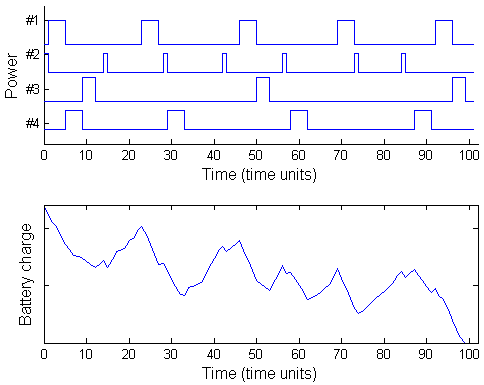
\includegraphics[scale=0.57]{edfbattery.png}
\caption{Schedule (top) and battery charge level (bottom) during simulation of \textsc{edf} algorithm.\label{fig:edfbattery}}
\end{center}
\end{figure}

\begin{figure}[tb]
\begin{center}
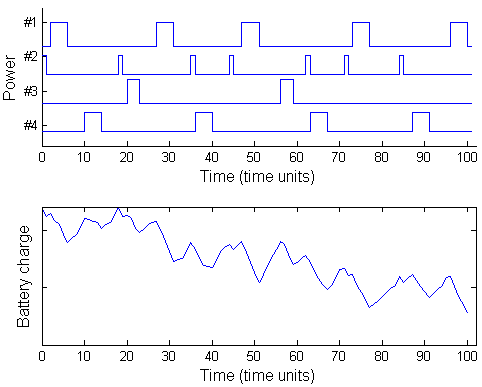
\includegraphics[scale=0.57]{edfstfubattery.png}
\caption{Schedule (top) and battery charge level (bottom) during simulation of \textsc{edf} algorithm on \textsc{stfu} tasks.\label{fig:edfstfubattery}}
\end{center}
\end{figure}

\begin{figure}[tb]
\begin{center}
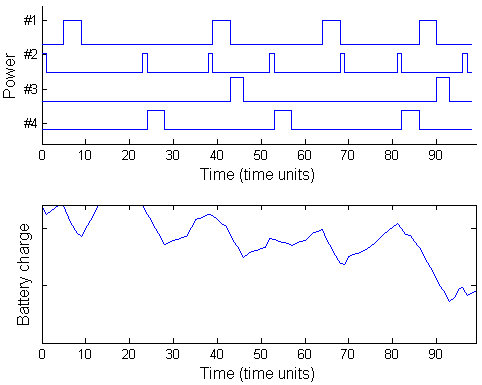
\includegraphics[scale=0.57]{lsabattery.png}
\caption{Schedule (top) and battery charge level (bottom) during simulation of static \textsc{lsa} algorithm.\label{fig:lsabattery}}
\end{center}
\end{figure}

\begin{figure}[tb]
\begin{center}
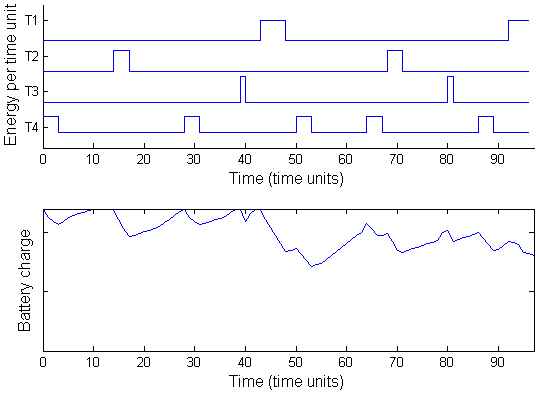
\includegraphics[scale=0.57]{lsastambattery.png}
\caption{Schedule (top) and battery charge level (bottom) during simulation of static \textsc{lsa} algorithm with \textsc{stam} tasks.\label{fig:lsastambattery}}
\end{center}
\end{figure}

Figures \ref{fig:edfbattery} to \ref{fig:lsastambattery} show the change in battery charge level when simulating a particular task list scheduled with four different algorithms.  
Figures \ref{fig:edfbattery} and \ref{fig:edfstfubattery} show the relative performance of plain \textsc{edf} and \textsc{edf} performed on \textsc{stfu} tasks.  The battery levels for the two simulations both have a downward trend at approximately the same rate, but in the \textsc{stfu} simulation the battery level rate of change is smoother.  
The large dip in charge that causes a violation at time 99 is ``filtered out'' by \textsc{stfu}, which gives the system a chance to collect more power and recover.  The smoothing effect is also demonstrated in figures \ref{fig:lsabattery} and \ref{fig:lsastambattery} for the static \textsc{lsa} algorithm with and without \textsc{stam}.




